%----------------------------------------------------------------
%
%  File    :  survey-images.tex
%
%  Author  :  Keith Andrews, IICM, TU Graz, Austria
% 
%  Created :  27 May 1993
% 
%  Changed :  03 Feb 2017
% 
%----------------------------------------------------------------


\chapter{Image Magnification}

\label{chap:images}

In this part of the project we have focused on presentation of images. We have 
added a zoom feature, which opens the clicked picture in a new window or in the 
enhanced version in a pop-up. The implementation works on different picture 
formats, of which we tested svg, jpeg, gif and png. Our enhancements give users 
a better opportunity to see detailed parts of the selected image, by fitting it 
to the width of the screen, while supporting zooming for smaller details or 
prefered size readjustment. Since zooming is involved and screen space is 
limited, we solve the overflow problem with scroll bars.

\begin{figure}[hp]
\centering

\subcaptionbox[Original Presentation Image Size]{%
Size of image set by the presentation creator.%
  
    \label{subfig:realy_img}%
}
[%
    0.44\hsize % width of caption
]%
{%
    \includegraphics[keepaspectratio,width=0.45\hsize]%
    {images/image1.png}%
}%
\hspace{0.05\hsize} % seperation
\subcaptionbox[Image Zoom For Detail] {%
   Zoomed-in part of same image.%
    \label{subfig:zoomed_img}%
}
[%
    0.44\hsize % width of caption
]%
{%
    \includegraphics[keepaspectratio,width=0.45\hsize]%
    {images/image2.png}%
}%
\caption[]{A SVG image inside the presentation before and after the 
magnification click.
\imgcredit{Screenshots taken by the authors of this report, while the original 
image is from a provided presentation \citep{keithDataVis}.
\label{fig:popup}
}}

\end{figure}

On click the selected image opens in a new tab or in the enhanced version in a 
pop-up window. While the complex pop-up function is provided by a 3rd party 
solution, the simplier new tab opening is done by supplying HTML content 
through JavaScript's document.write function on a new blank document. The 
provided content includes the page layout, buttons, the magnified picture, and 
JavaScript, which is needed for image resizing. To simplify the JavaScript 
inclusion, a seperate function is written, which is then converted to tex 
through the String function.

\begin{figure}[tp]
\centering
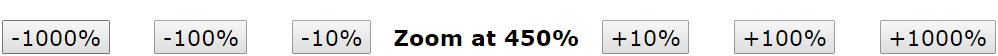
\includegraphics[keepaspectratio,scale=0.5]{images/button.png}

\caption[Image Magnification Controls]{
The magnification control bar next to the zooming buttons includes an updatable 
label, to report the current zoom in regards to original image size. 
\imgcredit{Screenshot taken by the authors of this report.}

}
\label{fig:Buttons}
\end{figure}

\newpage

In either the popup or tab window we can zoom it for +-10\%, +-100\%, and 
+-1000\% by pressing the provided buttons. Alternatively with keyboard or mouse 
support, we can also zoom it with +/- keyboard buttons or CTRL plus mouse 
scrolling event by a the default step of 10. To fit it back into the default 
size, where zoom is 100\%, we can do it by pressing keyboard button 0.

\begin{lstlisting}[
language=JavaScript,
label=openImgCode,
caption={[Image Magnification Initialization]%
Implementation of image detection and click event binding of content push. The 
called function is for the tab solution, while the pop-up solution seperates 
the control bar in the 3rd party sweetalert function call for layout 
improvement.
}
]
	  // Input listeners
		var images = document.getElementsByTagName("img");
		var images  = content_section.getElementsByTagName("img");

		for (var i=0, len=images.length, img; i<len; i++) {
		  img = images[i];
		  img.addEventListener("click", function() {
			openImageTab(this.src);
		  });
		}
	};
}

function openImageTab(imgSrc) {
	var newWindow = window.open();
	
	var htmlCode ="<head><title>rSlidy Image View</title><link 
rel='stylesheet' href='css/reset.css'><link rel='stylesheet' 
href='css/normalise.css'>" +
			"<link rel='stylesheet' href='css/rslidy.css'><link 
rel='stylesheet' href='css/slides-default.css'></head>" +
			"<body><div class='slide 
imageAlert'><h1><button>-1000\%</button><button>-100\%</button><button>-10\%</bu
tton>Zoom at <span 
id='zoomNumber'>100</span>\%<button>+10\%</button><button>+100\%</button><button
>+1000\%</button></h1>" +
			"<div><img id='zoomedImg' src='"+ imgSrc + 
"'></div></div>"+
			"<script type='text/javascript'>" + 
String(openImageTabListeners) + "; openImageTabListeners();</script></body>";
	newWindow.document.write(htmlCode);
}
\end{lstlisting}

\newpage

\begin{lstlisting}[
language=JavaScript,
label=imgControls,
caption={[Image Magnification Controls]%
	The control functions for all events are same for both rSlidy versions.
}
]
	
	window.addEventListener('keypress', function (e) {
		if (e.key == '+' || e.key == '-' || e.key == '0') {
			var zoom = parseInt(titleElement.innerHTML);
			if(e.key == '+'){
				zoom = zoom + 10;
			}
			else if(e.key == '-')
			{
				zoom = zoom - 10;
			}
			else{
				zoom = 100;
			}
			if(zoom > 0){
				img.style.height = zoom * heightPer + "px";
				img.style.width = zoom * widthPer + "px";
				titleElement.innerHTML = zoom;
			}
		}
	}, false);

	var isCtrl = false;
	window.addEventListener('keydown', function (e) {
		if (e.which === 17) {
            isCtrl = true;
        }
    }, false);
	window.addEventListener('keyup', function (e) {
		if (e.which === 17) {
            isCtrl = false;
        }
    }, false);

	window.addEventListener("mousewheel", function (e) {
		if(isCtrl){
			var delta = Math.max(-1, Math.min(1, e.wheelDelta));
			var zoom = parseInt(titleElement.innerHTML);
			if(delta > 0){
				zoom = zoom + 10;
			}
			else if(delta < 0)
			{
				zoom = zoom - 10;
			}
			if(zoom > 0){
				img.style.height = zoom * heightPer + "px";
				img.style.width = zoom * widthPer + "px";
				titleElement.innerHTML = zoom;
			}
		}
	}, false);
}
\end{lstlisting}